 %!TeX root = PHYS42 Lecture Notes.tex
\documentclass{article}
\usepackage[dvipsnames, svgnames, x11names]{xcolor}
\usepackage{tikz}
\usepackage{pgfplots}
\usepackage{pgfplotstable}
\usepackage{setspace}
\usepackage{units}
\usepackage{booktabs}
\usepackage{graphicx}
\usepackage{amsfonts}
\usepackage{circuitikz}
\usepackage{multirow}
\usepackage{amsopn}
\usepackage{bbding}
\usepackage{amsmath}
\usepackage{hyperref}
\usepackage{cancel}
\usepackage{gensymb}
\usepackage[margin = 1.2in]{geometry}

\newcommand{\midlabelline}[3]{
   \node (midlabel) at ($ (#1)!.5!(#2) $) {#3};
   \draw[latex-] (#1) --  (midlabel);
   \draw[-latex] (midlabel) -- (#2);
}

\AtBeginEnvironment{document}{\everymath{\displaystyle}}
\title{MATH 2 Lecture Notes}
\date{Tuesday, 14 January, 2025}
\author{Tejas Patel}
\begin{document}
\maketitle
\tableofcontents
\pagebreak
\section{Chapter 1}
\subsection{Terminology}
\textbf{Definition} A differential equation is an equation containing the derivatives or differentials 
of one or more dependent variables, with respect to one or more independent variables.\\
\textbf{$\cdot$} An Ordinary Differential Equation (ODE) involves only ordinary derivatives\\
\textbf{$\cdot$} A Partial Differential Equation (PDE) involves partial derivatives.\\
\textbf{Definition} The order of a DE is the order of the highest-order derivative that appears in the DE
\textbf{Notation} $F(x,y,\frac{dy}{dx}, \frac{d^2y}{dx^2})$\\
\textbf{Definition} A linear DE is any DE that can be written in form:\\
${\displaystyle a_{0}(x)y+a_{1}(x)y'+a_{2}(x)y''\cdots +a_{n}(x)y^{(n)}=b(x)}$\\
For a DE to be linear:
\begin{enumerate}
    \item Y and all of its derivatives much be of the 1st degree
    \item Any term that does not include y or any of its derivatives must be a function of x
\end{enumerate}
\subsection{Some Mathematical Models}
\subsubsection*{I. Free-falling body}
Goal: Find s(t). 
\\Set up a differential equation in S, model it, then solve
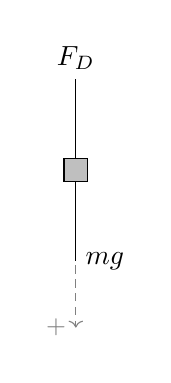
\begin{tikzpicture}[
    force/.style={>=latex,draw=blue,fill=blue},
    axis/.style={densely dashed,gray,font=\small},
    M/.style={rectangle,draw,fill=lightgray,minimum size=0.5cm,thin},
    m/.style={rectangle,draw=black,fill=lightgray,minimum size=0.3cm,thin},
    plane/.style={draw=black,fill=blue!10},
    string/.style={draw=red, thick},
    pulley/.style={thick},
]
\matrix[column sep=1cm] {
    \node[m] (m) {};

    \draw[axis,->] (m) -- ++(0,-2) node[left] {$+$};
    {[force,->]
    \draw (m.north) -- ++(0,1) node[above] {$F_D$};
        \draw (m.south) -- ++(0,-1) node[right] {$mg$};
    }
\\
};
\end{tikzpicture}\\
$ma=mg\\\frac{d^2s}{dt^2}=g\\v=\frac{ds}{dt}, g=\frac{dv}{dt}$\\
What if there is air resistance. Assume force scales linear with velocity
\\$\frac{dv}{dt}=g-\frac{kv}{m} \rightarrow \frac{dv}{dt}=g-\frac{k}{m}\cdot \frac{ds}{dt}$
\subsubsection*{II: Series Circuit}
\begin{circuitikz}
    \draw[line width=0.8]
     (2,7) to [sinusoidal voltage source, l_=$V_S$, i=$I$] (2,1)
     (2,7) to [resistor, l_=$R$] ++(6,0) to [inductor, l_=$L$] ++(0,-6) to [capacitor, l_=$C$] +(-6,0) ;
    \midlabelline{2,8}{8,8}{$V_R$}
    \midlabelline{9,7}{9,1}{$V_L$}
    \midlabelline{2,0}{8,0}{$V_C$}
\end{circuitikz}

Voltage drops:\\ $
V=L \frac{dI}{dt}, V=L \frac{d^2q}{dt^2}\\
V=IR, V= R \frac{dq}{dt}\\
V=\frac{q}{C}\\
E(t) = L \frac{d^2q}{dt^2}+ R \frac{dq}{dt} + \frac{q}{C}
$
\subsubsection*{III: Population Growth}
$P=P(t) =$ population at time t — use exponential model \\
$\frac{dp}{dt} \propto P \rightarrow \frac{dp}{dt} = kP \rightarrow = Ce^{kt}$ where C is the initial population
\subsubsection*{IV: Population Growth with Finite Capacity}
"Carrying Capacity" = N — uses the logistic growth model\\
$\frac{dp}{dt} \propto $ both P and amount to carrying capacity (N-P)\\
$\frac{dp}{dt}=kP(N-P)$
\subsubsection*{V: Chemical Reaction}
$A+B\rightarrow C$ Concentrations of A and B decreases by amount of C formed \\ 
Can we write DE governing the concentration of C x(t)? \\ 
The rate at which the reaaction takes place $\propto$ Product of the remaining concentrations of A and B
\\ $\alpha$ initial concentration of A
\\ $\beta$ initial concentration of B
\\ $\frac{dx}{dt} = k(\alpha - x)(\beta - x)$
\section{First-Order Differential Equations}
\subsection{Preliminary Theory}
Example DE: $y'=3y \Rightarrow \boxed{y=Ce^{3x}}$ the general solution where C is an arbitrary constant
\\[0.05in]Add initial condition $y(0) = 5$ plug in x=0 to $5=Ce^{3*0}, 5=C*1, C=5 \Leftarrow$ Initial Value Problem
\\$y=5e^{3x}$ is the general solution for the Initial Value Problem\\\subsubsection{\textbf{Theorem}}
$f(x) = \begin{cases}
    \frac{dy}{dx} = f(x,y) & \text{Differential Equation}\\
    y(x_0) = y_0  & \text{Initial Condition}
    \end{cases}$\\ Let R be a rectangular region in the xy-plane defined by $a\leq x \leq b, c \leq y \leq d $, that contains the point $(x_0, y_0)$ in its interior. \\[0.1in] If f(x,y) and $\frac{\partial f}{\partial y}$ are continuous on $R$, then there exists an interval I centered at $x_o$, and on this interval $I$ there exists a unique solution $y(x)$ for this IVP\\
\subsubsection{\textbf{Key Questions:}}Does every IVP have at least one solution?\\ If an IVP has a solution is it the only solution?

\textbf{Meaning of a solution existing "on an Interval"}
The initial value problem
\\$\begin{cases}
    \frac{dy}{dx} =1+y^2
    \\ y(0)=0
\end{cases}$ has a unique solution. In fact, we can easily verify that $y=\tan x$ satisfies this IVP
\\ However note that there are some inervals on which $y=\tan x$ cannot be a solution for this IVP, such as (-2,2),
where the function is discontinuous at $\pm \frac{\pi}{2}$ but can be used for (-1,1) since it is continuous at all points within the interval
\subsection{Separable Variables (Separable Equations)}
\subsubsection{\textbf{Definition: }}A differential equation that can be written in the form $\frac{dy}{dx}= \frac{g(x)}{h(y)}$ is said to be separable (or have separable variables).
\\\textbf{Example: } $\frac{dy}{dx}= \frac{g(x)}{h(y)} \\[0.05in]h(y) dy = g(x) dx \\[0.05in] \int{h(y)}{dy} = \int g(x) dx$ 
\\\textbf{Example: } $dx+e^{3x}dy=0$ \\ $e^{3x} dy = -dx$ \\ $dy=-\frac{dx}{e^{3x}}\rightarrow dy=-{e^{-3x}}{dx} \rightarrow \int dy=\int -{e^{-3x}}{dx} \rightarrow y=\frac{1}{3}e^{-3x}+C$ where C is an arbitrary constant
\subsubsection{Substitution} $\frac{dy}{dx} = F(ax+bc+c)$ where $b\neq 0$ use the substitution: $u=ax+by+c \Rightarrow \frac{du}{dx} = a+b\frac{dy}{dx} = \frac{1}{b}\left[\frac{du}{dx}-a\right]$
\\Example: $\frac{dy}{dx} = \tan^2(x+y)$ let $u=x+y \rightarrow \frac{dy}{dx}=\frac{du}{dx}-1 \rightarrow \frac{du}{dx}-1=\tan^2 u \rightarrow \frac{du}{dx} = \sec ^2 u \\ \int \cos^2 u \; du = \int dx \\ 2(x+y)+\sin2(x+y) = 4x+C \rightarrow 2y-2x+\sin2(x+y)$
\\ \textbf{Solve:}
$\frac{dy}{dx} = (y+3)^2$ By inspection $y=-3$ is a solution. This is the only solution because $f(x,y)=(x+3)^2$ is continuous on $\mathbb{R}^2$ and $\frac{\partial f}{\partial x}$ is continuous on$ \mathbb{R}$ so it is the only solution
Why solving by separation is not possible
$\int (y+3)^-2 dy=\int dx \rightarrow (y+3)^-2/-1=x+C_1 \rightarrow \frac{1}{y+3}=-x-C_1 \rightarrow y+3 = \frac{1}{c-x} \rightarrow y=-3+\frac{1}{c-x}
\\y(0)=-3\rightarrow 0=\frac{1}{c}$ where there is no real c that solves that equation, making this not possible
\subsection{Homogeneous Equations} 
\textbf{What do we do if the DE is not separable?}
\subsubsection{Definition} A function $f(x,y)$ is said to be \textbf{homogeneous of degree} $n$ if, for $x, y,$ and$ t $where $f(x,y)$ and $f(tx,ty)$ are defined: \\$$f(tx,ty)=t^nf(x,y)$$
\subsubsection{Example} Determine wheteher each function is homogeneous: \\
a: $ f(x,y)=x^3-7x^2y+4y^3 \rightarrow f(tx,ty)=(tx^3)-7(tx)^2(ty)+4(ty)^3\\t^3x^3-7t^3x^2y+4t^3y^3\\t^3(x^3-7x^2y-4y^3)=t^3f(x,y)$
\\How to tell quickly wheteher $f(x,y)$ is homogeneous:
\\Each term must have the same combined degree
\\Example: $x^3-7x^2y+4y^3$ is D3, $x^2+y^2-4x$ is not, $\sqrt{x^5+4y^5}$ is with D 2.5, $\frac{3y}{x}-2$ is D0
\subsubsection{Differential Equation form}
$M(x,y)dx+N(x,y)dy=0$ is called a homogeneous differential equation if the functions $M$ and $N$ are both homogeneous of the same degree
\\If $f(x,y)$ is homogeneous of degree $n$ then $f(x,y)$ can be written as:
\\$f(x,y)=f(x\times 1, x \times \frac{y}{x})=x^nf(1, \frac{y}{x})$
\\or $f(x,y)=y^nf(\frac{x}{y},1)$
\subsubsection{Substitution} to solve a homogeneous DE make the substitution: $y=ux \;\; (u=\frac{y}{x})$ or$ x=vy \; \; (v=\frac{x}{y})$
\subsubsection{Example}
$(y^2+xy)dx+x^2dy=0 \rightarrow y=ux \rightarrow dy=(udx+xdu) \\ (u^2x^2+ux^2)dx+x^2(udx+xdU)=0\\u^2x^2dx+ux^2dx+ux^2dx+x^3du=0 \\ ux^2(u+2)dx+x^3du=0\\\int \frac{1}{u(u+2)}du=-\int \frac{1}{x}dx \\$ Partial Fraction Decomposition: $\frac{1}{u(u+2)}=\frac{A}{u}+\frac{B}{u+2} \rightarrow A=\frac{1}{2}, B=-\frac{1}{2}$ Back to solving \\ $\int \left[\frac{0.5}{u}-\frac{0.5}{u+2}\right]=-\int \frac{1}{x} dx \\ 0.5\ln|u|-1/2 \ln |u+2|=-\ln |x|+C_1 \\ \ln \left|\frac{u}{u+2}\right|=2C_1-2\ln|x| \\ \left|\frac{u}{u+2}\right|=e^{2C_1}\cdot e^{-2\ln|x|} = e^{2C_1}\cdot |x^{-2}| \Rightarrow \left|\frac{u}{u+2}\right| = \left|e^{2C_1}\cdot x^{-2}\right| \Rightarrow \left|\frac{u}{u+2} = \frac{C}{x^2}\right| \\ ux^2=X(u+2) \Rightarrow ux^2=Cu+2c \rightarrow ux^2-Cu=2C \\ u(x^2-c)=2C \Rightarrow u= \frac{2C}{x^2-C} \Rightarrow \frac{y}{x} = \frac{2Cx}{x^2-C}, \; x \neq 0$
\subsection{Exact Equations}
\subsection{Preliminary Theory}














\pagebreak
\section{Example Problems with Solutions}
\subsection{}
$\begin{cases}
    \frac{dy}{dx} = 2xy^\frac{2}{3}\\
    y(0) = 0  \\
\end{cases}$
$y=0$ and $y=\frac{x^6}{27}$ are solutions \\[0.05in]$\frac{dy}{dx} \frac{x^6}{27} = 2x \cdot \frac{x^4}{9} = y^\frac{2}{3}$
\\[0.05in]$\begin{cases}
    \frac{dy}{dx} = 2yx^\frac{2}{3}\\
    y(0) = 0  \\[0.05in]
\end{cases}$ and $y=0$ is the only solution. This IVP satisfies a certain condition and that makes it have a unique solution
\\[0.05in]$\begin{cases}
    \frac{dy}{dx} = xy^\frac{1}{2}\\
    y(0) = 0  \\
\end{cases}$
\\ Does the IVP have a unique solution? When on $\mathbb{R}^2$ is $\frac{\partial f}{\partial y}$ continuous? $\frac{\partial f }{ \partial y }= \frac{1}{2} xy^{-\frac{1}{2}} = \frac{x}{2\sqrt{y}}$
\\$\begin{cases}
    \frac{dy}{dx} = 3y\\
    y(0) = 5  \\
\end{cases}$ 
Yes there is a unique solution, $\frac{\partial f}{\partial y} = 3$\\
Determine the region R for which the DE would have a unique solution through a point $(x_0, y_0)$ in the region
$\frac{dy}{dx} = \sqrt{xy}$ \\ Where on $\mathbb{R}^2$ is $\frac{\partial f}{\partial y}$ continuous? $\frac{\partial f}{\partial y} = \frac{1}{2}(xy)^{-1/2} * \frac{\partial}{\partial y} (xy) = \frac{x}{2\sqrt{xy}}$
\\ \textbf{DIY}
\\ $\frac{dy}{dx}-y=x$ 
\subsection{}
\textbf{Solve: } $ydx=(2+3x)dy$ \\ $\frac{dy}{y} = \frac{dx}{2+3x}$ \\ $\int \frac{dy}{y} = \int \frac{dx}{2+3x}$ \\ $\ln |y| = \frac{ \ln |2+3x|}{3} + C$  \\ $e^{\ln |y|} = e^{\frac{ \ln |2+3x|}{3} + C_1}$ 
\\ $=  e^{\frac{ \ln |2+3x|}{3}} \cdot e^{C_1}$ \\ $|y| = e^{C_1} \cdot {\ln |2+3x| ^ {\frac{1}{3}}}$ \\ $|y| = \left|e^{C_1}\right| \cdot \left|(2+3x)^{^\frac{1}{3}}\right|$\\ $|y| = \left|e^{C_1} \cdot |(2+3x)^{^\frac{1}{3}}\right|$ \\ $y = \pm C(2+3x)^{^\frac{1}{3}} \qquad x \neq -\frac{2}{3}$
\subsection{}
$\frac{dy}{dx} = e^xe^{5y} \\ e^{-5y}dy = \frac{e^x}{dx} \\ \int e^{-5y}dy = \int e^x dx \\ -\frac{1}{5}e^{-5y} = e^x + C_1 \\ 
e^{-5y}=-5e^x-5C_1 \\ -5y=\ln(-5e^x-5C_1) \\ y= -\frac{1}{5}\ln(C-5e^x)$
\subsection{}
$y'=2y-y^2 \\ \frac{dy}{dx} = y(2-y) \rightarrow \int \frac{dy}{y(2-y)} = \int dx \rightarrow \int \left(\frac{0.5}{y} + \frac{0.5}{2-y}\right) dy=\int dx \\ \frac{1}{2}\ln|y| - \frac{1}{2}\ln|2-y| = x+C_1 \\ \ln|y| - \ln |2-y| = 2x+2C_1
\\ \ln \left|\frac{y}{2-y}\right| = 2x+2C_1 \Rightarrow \left|\frac{y}{2-y}\right| = e^{2x}e^{2C_1} \rightarrow \frac{y}{2-y} = Ce^{2x} \rightarrow y=CE^{2x}(2-y) \\ y=2Ce^{2x}-Ce^{2x}y \rightarrow (1+Ce^{2x})y=2Ce^{2x} \\ \boxed{y=\frac{2Ce^{2x}}{1+Ce^{2x}}} \rightarrow \frac{2C}{e^{-2x}+C}$
\subsection{}
$(x-y)dx+xdy=0$
\\Substitution $y=ux \Rightarrow dy=udx+xdu$
\\$(x-ux)dx+x(udx+xdu)=0 \\ xdx-uxdx+uxdx+x^2du=0 \\ xdx+x^2du=0 \\ \int du= -\int \frac{1}{x}dx \Rightarrow u=-\ln |x|+C \\ u=\frac{y}{x} \\ \frac{y}{x}=C-\ln|x| \\ y=Cx-x\ln |x|$

\end{document}